\documentclass[onecolumn]{article}
\usepackage{url}
\usepackage{algorithmic}
\usepackage[a4paper]{geometry}
\usepackage{datetime}
\usepackage[margin=2em, font=small,labelfont=it]{caption}
\usepackage{graphicx}
\usepackage{mathpazo} % use palatino
\usepackage[scaled]{helvet} % helvetica
\usepackage{microtype}
\usepackage{amsmath}
\usepackage{amssymb}
\usepackage{enumitem} % alphabetic enumeration
\usepackage{lmodern}
\usepackage[T1]{fontenc}
\usepackage{subfigure}
% Letterspacing macros
\newcommand{\spacecaps}[1]{\textls[200]{\MakeUppercase{#1}}}
\newcommand{\spacesc}[1]{\textls[50]{\textsc{\MakeLowercase{#1}}}}

\def\doubleunderline#1{\underline{\underline{#1}}}

\title{\spacecaps{Lab report: SW02 }\\ \normalsize \spacesc{TSM\_DeLearn} }

\author{Andrin Bürli\thanks{andrin.buerli@hslu.ch}, Nursinem Dere\thanks{nursinem.dere@stud.hslu.ch}, Fabian Gröger\thanks{fabian.groeger@hslu.ch}\\Hochschule Luzern}
\date{\today}

\begin{document}
\maketitle

\section{Exercise 2}

\subsection{Task (a)}

\[
\begin{aligned}
	\sigma(z)&=\frac{1}{1+e^{-z}}\\
	\frac{d}{dz} \sigma(z) &= \frac{d}{dz}(1+e^{-z})^-1=-(1+e^{-z})^{-2}(-e^{-z})=\frac{e^{-z}}{(1+e^{-z})^{2}}
\end{aligned}
\]

\subsection{Task (b)}

\[
\begin{aligned}
	\sigma(z)&=\frac{1}{1+e^{-z}} \\
	\frac{d}{dz} \sigma(z) &= \frac{e^{-z}}{(1+e^{-z})^{2}}=\frac{1+e^{-z}-1}{(1+e^{-z})^{2}} \\
	&=\sigma(z)^2(1+e^{-z}-1)=\sigma(z)^2(\sigma(z)^{-1}-1) \\
	&=\sigma(z)(1-\sigma(z))
\end{aligned}
\]

\subsection{Task (c)}

\[
\begin{aligned}
	\zeta(z)&=-\text{log}(\sigma(-z))=-\text{log}\left(\frac{1}{1+e^z}\right)\\
	\\
	\frac{d}{dz} \zeta(z) &= -\frac{1}{\sigma(-z)} \sigma(-z)(1-\sigma(-z))\cdot (-1) = (1-\sigma(-z)) \\
	\\
	\frac{d^2}{dz^2} \zeta(z) &=\frac{d}{dz} (1-\sigma(-z))=-(-\sigma(-z)(1-\sigma(-z)))\\
	&=\sigma(-z)(1-\sigma(-z))
\end{aligned}
\]
Now in order to find the boundaries we let the variable $z$ run to infinity in both directions

\[
\begin{aligned}
	\lim_{z\to+\infty}\zeta(z)&=	\lim_{z\to+\infty}-\text{log}\left(\frac{1}{1+e^\infty}\right)
	=\lim_{z\to+\infty}-\text{log}\left(\frac{1}{\infty}\right)
	=\lim_{z\to+\infty}-\text{log}\left(0\right)=\infty \\
	\lim_{z\to-\infty}\zeta(z)&=\lim_{z\to-\infty}-\text{log}\left(\frac{1}{1+e^{-\infty}}\right)
	=\lim_{z\to-\infty}-\text{log}\left(\frac{1}{1+0}\right)
	=\lim_{z\to-\infty}-\text{log}\left(1\right)=0
\end{aligned}
\]
\begin{figure}[hbt!]
	\centering
	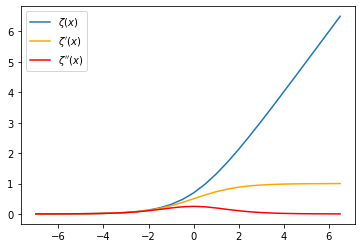
\includegraphics[width=.6\linewidth]{taskc.png}
	\caption{The $\zeta(z)$ function and its derivatives}
\end{figure}

\subsection{Task (d)}
\begin{figure}[hbt!]
	\centering
	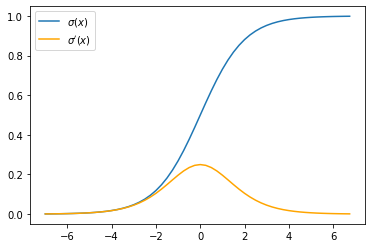
\includegraphics[width=.6\linewidth]{taskd.png}
	\caption{The logistic / sigmoid function $\sigma(x)=\frac{1}{1+e^{-x}}$ function and its first derivative}
\end{figure}

\subsection{Task (f)}
\label{taskf}
\[
\begin{aligned}
	c_1(x)=SE(x) &= (\sigma(x)-1)^2 \\
	\\
	\frac{d}{d x} SE(x)&= 2(\sigma(x)-1)\sigma(x)(1-\sigma(x))=2\sigma(x)(\sigma(x)-1) (1-\sigma(x)) \\
	&=2\sigma(x)(\sigma(x)-\sigma(x)^2-1+\sigma(x))=-2\sigma(x)(\sigma(x)^2-2\sigma(x)+1) \\
	&=-2\sigma(x)(\sigma(x)-1)^2 \\
	\\
	\frac{d^2}{d x^2} SE(x)&=-2\sigma(x)(1-\sigma(x))(\sigma(x)-1)^2-2\sigma(x)2(\sigma(x)-1)\sigma(x)(1-\sigma(x))\\
	&=-2\sigma(x)(1-\sigma(x))((\sigma(x)-1)^2+2\sigma(x)(\sigma(x)-1)) \\ &=-2\sigma(x)(1-\sigma(x))(\sigma(x)-1)(\sigma(x)-1+2\sigma(x)) \\
	&=2\sigma(x)(\sigma(x)-1)^2(3\sigma(x)-1) \\
	&=\sigma(x)(\sigma(x)-1)^2(6\sigma(x)-2) 
	\\ \\
	\sigma(x)&\to(0, 1) \\
	(\sigma(x)-1)^2&\to(0,1) \\
	(6\sigma(x)-2) &\to \left\{\begin{array}{lr}
		[0, -2), & \text{for } x \leq -\text{ln}(2) \\
		(0, 4), & \text{for } x > -\text{ln}(2)
	\end{array}\right\} \to \text{hence SE is non convex}
\end{aligned}
\]\\
If we start at some initial point $x_0 << 0$ we will have a gradient that is very close to zero because

\[
\lim_{x\to-\infty}{\frac{d}{d x} SE(x)}=\lim_{x\to-\infty}{-2\sigma(x)(\sigma(x)-1)^2 }=\lim_{x\to-\infty}{-2\sigma(-\infty)(\sigma(-\infty)-1)^2 }=\lim_{x\to-\infty}{-2\cdot 0(0-1)^2 }=0
\]

Hence the gradient update step $x_{t}\leftarrow x_{t-1}-\frac{d}{dx}SE(x_{t-1})$ will push the algorithm only very little into the correct direction. That direction will still minimize the squared error $c_1$, but it will do so very slowly. This phenomenon is also known as the vanishing gradient problem.
\begin{figure}[hbt!]
	\centering
	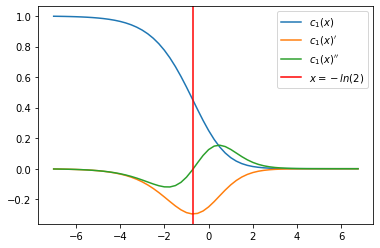
\includegraphics[width=.5\linewidth]{taskf.png}
	\caption{The squared error $c_1$ with its derivatives and a vertical line at the threshold where the second derivative enters the positive range.}
\end{figure}

\subsection{Task (g)}
\[
\begin{aligned}
	c_{2}(x)=CE(x)&=-(y \log (\sigma(w \cdot x))+(1-y) \log (1-\sigma(w \cdot x))) \\ \\
	\frac{\partial}{\partial w} CE(x)&=\frac{\partial}{\partial w}-\left(y\log \sigma(wx)+(1-y) \log \left(1-\sigma(wx)\right)\right)=-\left(\frac{y}{\sigma(wx)}\sigma(wx)^\prime x-\frac{1-y}{1-\sigma(wx)}\sigma(wx)^\prime x\right) \\
	&=-\sigma(wx)^\prime x\left(\frac{y}{\sigma(wx)}-\frac{1-y}{1-\sigma(wx)}\right)=-\sigma(wx)^\prime x\left(\frac{y(1-\sigma(wx))-(1-y)\sigma(wx)}{\sigma(wx)^\prime}\right) \\
	&=x(\sigma(wx)-y) \\
	\\
	\frac{\partial^2}{\partial w^2} CE(x) &= \frac{\partial}{\partial w} x(\sigma(wx)-y) = \sigma^\prime(wx) x^2 \\
	&= \sigma(wx)(1-\sigma(wx)) x^2 \\
	\\ \\
	\sigma(wx)&\to(0,1) \\
	(1-\sigma(wx))^2&\to(0,1) \\
	x^2 &\to (0, \infty) \text{ for } x\neq0 \to \text{hence } CE(x) \text{ is convex}
\end{aligned}
\]

\section{Exercise 4}
\subsection{Task a}
It is beneficial because the input features are scaled similarly and thus build a loss landscape that is easier to optimize. Otherwise, the model additionally needs to learn to cope with the different feature scales, which leads to longer training and poorer performance. the scales before learning the actual importance of the features for the task at hand.

\subsection{Task b}
Machine learning optimization is the process of adjusting the hyperparameters in order to
minimize the cost function by using one of the optimization techniques. It is important to
minimize the cost function because it describes the discrepancy between the true value of
the estimated parameter and what the model has predicted.

\subsection{Task c}
Gradient descent can be applied as soon as a problem can be defined as the optimization of a continuous and differentiable function. It is a local algorithm and will only lead to a unique solution if the given function is also convex ($f^{\prime\prime}(x)>0, x \in {\rm I\!R}^n$). If the function is not convex, the GD algorithm can easily get caught up in a local maxima as the gradient will converge to $0$ at such points.

\subsection{Task d}
The MSE function is non-convex for binary classification. If a binary classification model is trained with MSE Cost function, it is not guaranteed to minimize the Cost function. This is because MSE function expects real-valued inputs in range $(-\infty, +\infty)$, while binary classification models output probabilities in range (0,1) through the sigmoid/logistic function.

\subsection{Task e}
If the learning rate is too large, it can jump over the minima we are trying to reach, we
overshoot. This can lead to osculations around the minimum or in some cases to outright
divergence.

\subsection{Task f}
If that happens, the choosen parameters overfit the training data and do not well generalize to yet unseen datapoints.

\subsection{Task g}
It is harder to reach a small train error because the dataset incorporates more variance. But it is easier to have a smaller generalization error when having a larger dataset since it is assumed that the dataset gets more similar to the true underlying distribution.order to account for the additional variance in the larger training set.

\end{document}

